\documentclass[titlepage, a4paper]{article}
\usepackage[swedish]{babel}
\usepackage[utf8]{inputenc}
\usepackage{color}
\usepackage{graphicx}
\usepackage{etoolbox}
\usepackage{stringenc}
\usepackage{pdfescape}

% Sidformat
\usepackage{a4wide}

% Fixa Appendix-titlar
\usepackage[titletoc,title]{appendix}

% Bättre tabeller
\usepackage{tabularx}

% Bättre bildtexter
\usepackage[margin=10pt,font=small,labelfont=bf,labelsep=endash]{caption}

% Enkelt kommando som låter mig attgöra-markera text
\newcommand{\todo}[1] {\textbf{\textcolor{red}{#1}}}

% Nytt \paragraph låter oss ha onumrerade bitar
\makeatletter
\renewcommand\paragraph{\@startsection{paragraph}{4}{\z@}%
{-3.25ex\@plus -1ex \@minus -.2ex}%
{1.5ex \@plus .2ex}%
{\normalfont\normalsize\bfseries}}
\makeatother

%\providecommand{\LIPSlogga}{../mall/logga1.png}
\providecommand{\LIPSdatum}{\today}

%% Headers och Footers
\usepackage{fancyhdr}
\pagestyle{fancy}
%\lhead{\includegraphics[scale=0.4]{\LIPSlogga}}
\rhead{\ifdef{\LIPSutfardare}{Utfärdat av \LIPSutfardare \\\LIPSdatum}\LIPSdatum}
\lfoot{\LIPSkursnamn \\ \LIPSdokumenttyp}
\cfoot{\thepage}
\rfoot{\LIPSprojektgrupp \\ \LIPSprojektnamn}

%% Titelsida
\newcommand{\LIPSTitelsida}{%
{\ }\vspace{45mm}
\begin{center}
  \textbf{\Huge \LIPSdokument}
\end{center}
\begin{center}
  {\Large Redaktör: \LIPSredaktor}
\end{center}
\begin{center}
  {\Large \textbf{Version \LIPSversion}}
\end{center}
\vfill
\begin{center}
  {\large Status}\\[1.5ex]
  \begin{tabular}{|*{3}{p{40mm}|}}
    \hline
    Granskad & \LIPSgranskare & \LIPSgranskatdatum \\
    \hline
    Godkänd & \LIPSgodkannare & \LIPSgodkantdatum \\
    \hline
  \end{tabular}
\end{center}
\newpage
}

% Projektidentitet
\newenvironment{LIPSprojektidentitet}{%
{\ }\vspace{45mm}
\begin{center}
  {\Large PROJEKTIDENTITET}\\[0.5ex]
  {\small
  \LIPSartaltermin, \LIPSprojektgrupp\\
  Linköpings Tekniska Högskola, IDA
  }
\end{center}
\begin{center}
  {\normalsize Gruppdeltagare}\\
  \begin{tabular}{|l|l|p{25mm}|l|}
    \hline
    \textbf{Namn} & \textbf{Ansvar} & \textbf{Telefon} & \textbf{E-post} \\
    \hline
}%
{%
    \hline
  \end{tabular}
\end{center}
\begin{center}
  {\small
    \ifdef{\LIPSgruppadress}{\textbf{E-postlista för hela gruppen}: \LIPSgruppadress\\}{}
    \ifdef{\LIPSgrupphemsida}{\textbf{Hemsida}: \LIPSgrupphemsida\\[1ex]}{}
    \ifdef{\LIPSkund}{\textbf{Kund}: \LIPSkund\\}{}
    \ifdef{\LIPSkundkontakt}{\textbf{Kontaktperson hos kund}: \LIPSkundkontakt\\}{}
    \ifdef{\LIPSkursansvarig}{\textbf{Kursansvarig}: \LIPSkursansvarig\\}{}
    \ifdef{\LIPShandledare}{\textbf{Handledare}: \LIPShandledare\\}{}
  }
\end{center}
\newpage
}
\newcommand{\LIPSgruppmedlem}[4]{\hline {#1} & {#2} & {#3} & {#4} \\}

%% Dokumenthistorik
\newenvironment{LIPSdokumenthistorik}{%
\begin{center}
  Dokumenthistorik\\[1ex]
  %\begin{small}
    \begin{tabular}{|l|l|p{60mm}|l|l|}
      \hline
      \textbf{Version} & \textbf{Datum} & \textbf{Utförda förändringar} & \textbf{Utförda av} & \textbf{Granskad} \\
      }%
    {%
			\hline
    \end{tabular}
  %\end{small}
\end{center}
}

\newcommand{\LIPSversionsinfo}[5]{\hline {#1} & {#2} & {#3} & {#4} & {#5} \\}

% Kravlistor
\newenvironment{LIPSkravlista}{
	\center
		\tabularx{\textwidth}{| p{1.2cm} | p{1.9cm} | X | c |}
			\hline
			\textbf{Krav} & \textbf{Förändring} & \textbf{Beskrivning} & \textbf{Prioritet} \\\hline
}
{
		\endtabularx
	\endcenter
}

\newcounter{LIPSkravnummer}
\addtocounter{LIPSkravnummer}{1}
\newcommand{\LIPSkrav}[4][Krav \arabic{LIPSkravnummer}]{{#1} & {#2} & {#3} & {#4} \stepcounter{LIPSkravnummer}\\\hline}


% Leveranskravlistor
\newenvironment{LIPSleveranskravlista}{
	\center
		\tabularx{\textwidth}{| p{1.2cm} | p{1.9cm} | X | X |}
			\hline
			\textbf{Krav} & \textbf{Förändring} & \textbf{Beskrivning} & \textbf{Deadline}\\\hline
}
{
		\endtabularx
	\endcenter
}

\newcounter{LIPSleveranskravnummer}
\addtocounter{LIPSleveranskravnummer}{1}
\newcommand{\LIPSleveranskrav}[4][Krav \arabic{LIPSkravnummer}]{{#1} & {#2} & {#3} & {#4} \stepcounter{LIPSkravnummer}\\\hline}


% Milstolps-lista
\newenvironment{LIPSmilstolpar}{
	\center
		\tabularx{\textwidth}{| p{1.2cm} | X | l |}
			\hline
			\textbf{Nr} & \textbf{Beskrivning} & \textbf{Datum} \\\hline
}
{
		\endtabularx
	\endcenter
}

\newcounter{LIPSstolpnummer}
\addtocounter{LIPSstolpnummer}{1}
%\newcommand{\LIPSmilstolpe}[3][Krav \arabic{LIPSstolpnummer}]{{#1} & {#2} & {#3} \stepcounter{LIPSstolpnummer}\\\hline}
\newcommand{\LIPSmilstolpe}[3]{{#1} & {#2} & {#3} \\\hline}

% Aktivitets-lista
\newenvironment{LIPSaktivitetslista}{
	\center
		\tabularx{\textwidth}{| p{0.3cm} | X | c | c | c |}
			\hline
			\textbf{Nr} & \textbf{Beskrivning} & \textbf{Beroende av} & \textbf{Timmar} & \textbf{datum} \\\hline
}
{
		\endtabularx
	\endcenter
}

\newcounter{LIPSaktivitetsnummer}
\addtocounter{LIPSaktivitetsnummer}{1}
% \newcommand{\LIPSaktivitet}[4][\arabic{LIPSstolpnummer}]{{#1} & {#2} & {#3} & {#4} \stepcounter{LIPSstolpnummer}\\\hline}
\newcommand{\LIPSaktivitet}[5]{{#1} & {#2} & {#3} & {#4} & {#5}\\\hline}

% Mall för mötesprotokoll
\newenvironment{projektmote}[2]{
  {\ }\vspace{5mm}

  \centerline{\textbf{\Huge #1}}
  \vspace{2mm}
  \centerline{\LARGE #2}
  \vspace{10mm}

  \begin{itemize}
}
{
  \end{itemize}
}

\newcounter{paragrafnummer}
\addtocounter{paragrafnummer}{1}
\newcommand{\paragraf}[1]{\item{\textsection \arabic{paragrafnummer}. {#1}}\addtocounter{paragrafnummer}{1}}

% Mall för Statusrapport
\newenvironment{statusrapport}{
  \center
    \tabularx{\textwidth}{| p{0.4cm} | X | X | p{14.5mm} | p{13.5mm} | p{16.5mm} | p{16.5mm} |}
    \hline
    \textbf{Nr} & \textbf{Aktivitet} & \textbf{Beroenden} & \textbf{Planerad tid} & \textbf{Nedlagd tid} & \textbf{Planerad klar} & \textbf{Beräknat klart} \\\hline
}
{
    \endtabularx
  \endcenter
}

\newcommand{\aktivitetstatus}[7]{{#1} & {#2} & {#3} & {#4} & {#5} & {#6} & {#7} \\\hline}	% Importera generella layout-strukturer

% Information nödvändig för generella layout-strukturer
\newcommand{\LIPSredaktor}{Johannes Klasson}
\newcommand{\LIPSversion}{P1A}
\newcommand{\LIPSdokument}{Final Project Report}
\newcommand{\LIPSdokumenttyp}{Final Project Report}
\newcommand{\LIPSgranskatdatum}{2016-05-26}
\newcommand{\LIPSgranskare}{Johannes Klasson}
\newcommand{\LIPSgodkannare}{Martin Nielsen-Lönn}
\newcommand{\LIPSgodkantdatum}{-}
\newcommand{\LIPSkursnamn}{TSEK06}
\newcommand{\LIPSprojektnamn}{16-bit Kogge-Stone Adder}
\newcommand{\LIPSprojektgrupp}{Group 5}
\newcommand{\LIPSartaltermin}{VT, 2016}
\newcommand{\LIPSkund}{ISY}
\newcommand{\LIPSkundkontakt}{Martin Nielsen-Lönn}
\newcommand{\LIPSkursansvarig}{Atila Alvandpour}
\newcommand{\LIPShandledare}{Martin Nielsen-Lönn}

% Dokument-specifika paket
\usepackage{tabularx}
\usepackage{pdfpages}
\usepackage{tikz}
\usepackage{float}
\usetikzlibrary{shapes, arrows}
\usepackage{booktabs} % Horizontal rules in tables
\usepackage[justification=centering]{caption}
\usepackage{adjustbox}
\usepackage{siunitx}
\pagenumbering{roman}


\DeclareGraphicsRule{.0.pdf}{pdf}{*}{}

\begin{document}
\pagenumbering{gobble}
\LIPSTitelsida
\pagenumbering{gobble}
\begin{LIPSprojektidentitet}
  \LIPSgruppmedlem{Johan Isaksson}{Project Leader}{070-2688785}{johis024@student.liu.se}
  \LIPSgruppmedlem{Johannes Klasson}{Document Manager}{073-8209003}{johkl226@student.liu.se}
  \LIPSgruppmedlem{Jonas Tarassu}{VLSI Designer}{070-5738583}{jonta760@student.liu.se}
  \LIPSgruppmedlem{Alexander Yngve}{VLSI Designer}{076-2749762}{aleyn573@student.liu.se}	
\end{LIPSprojektidentitet}

\newpage
\pagenumbering{gobble}
\tableofcontents	%Innehållsförteckning
%\listoffigures
%\listoftables

\newpage
\pagenumbering{gobble}
\begin{LIPSdokumenthistorik}
\LIPSversionsinfo{P1A}{2016-05-26}{First draft}{Johan Isaksson}
\end{LIPSdokumenthistorik}

\newpage
\pagenumbering{arabic}	%Påbörja sidnumrering

% Inledning, översikt osv

\section{Introduction}
This document describes the state of the 16-bit Kogge-Stone adder project in the course TSEK06 after finishing the high level design phase. The system itself is supposed to receive two numbers that should be added together. The result should then both sent out from the system and be compared with a checksum in a BIST (Built-In Self-Test). The meaning of high level is that every basic logic gate is implemented in Verilog-A. The main reason for doing this is to be able to simulate all logic to make sure that everything works as intended. Block level diagrams can be found in section \ref{sec:block_level}, simulation results in section \ref{sec:simulation_results} and a risk analysis in section \ref{sec:risks}. In appendix \ref{app:time_plan} and \ref{app:time_report} a time plan of the next phase and a time report of this phase can be found.


\section{Project Description} \label{sec:project_description}
Much of the block level descriptions can be seen in the high level report, but the transistor view of the leaf-cells will be described in this chapter. To find good sizes for our gates we used a very simple sizing strategy. Start small, and if the signal is to weak to drive the components, we just size it up and if necessary, make a buffer for it. The transistor schematic of the basic blocks like AND, OR, DFF etc. are simple enough to leave out the description for them. In Fig. \ref{block_second} an updated block diagram of the complete system can be seen.

\begin{figure}[H]
  \centering
  \captionsetup{justification=centering}
  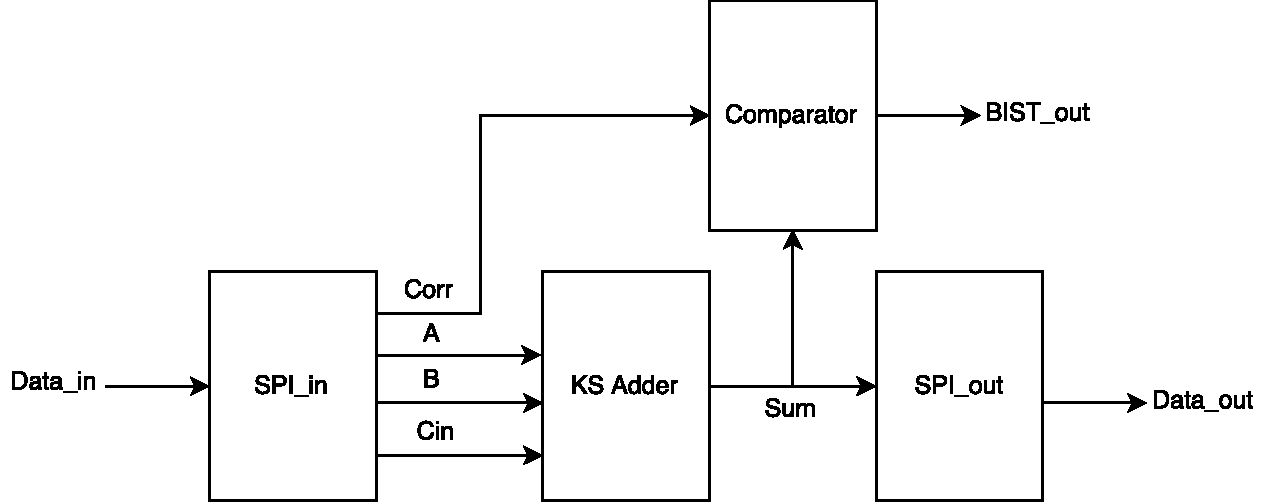
\includegraphics[scale=0.5]{../figures/TOP.pdf}
  \caption{Block diagram of the system first iteration.} \label{fig:block_first}
\end{figure}

\begin{figure}[H]
\centering
\captionsetup{justification=centering}
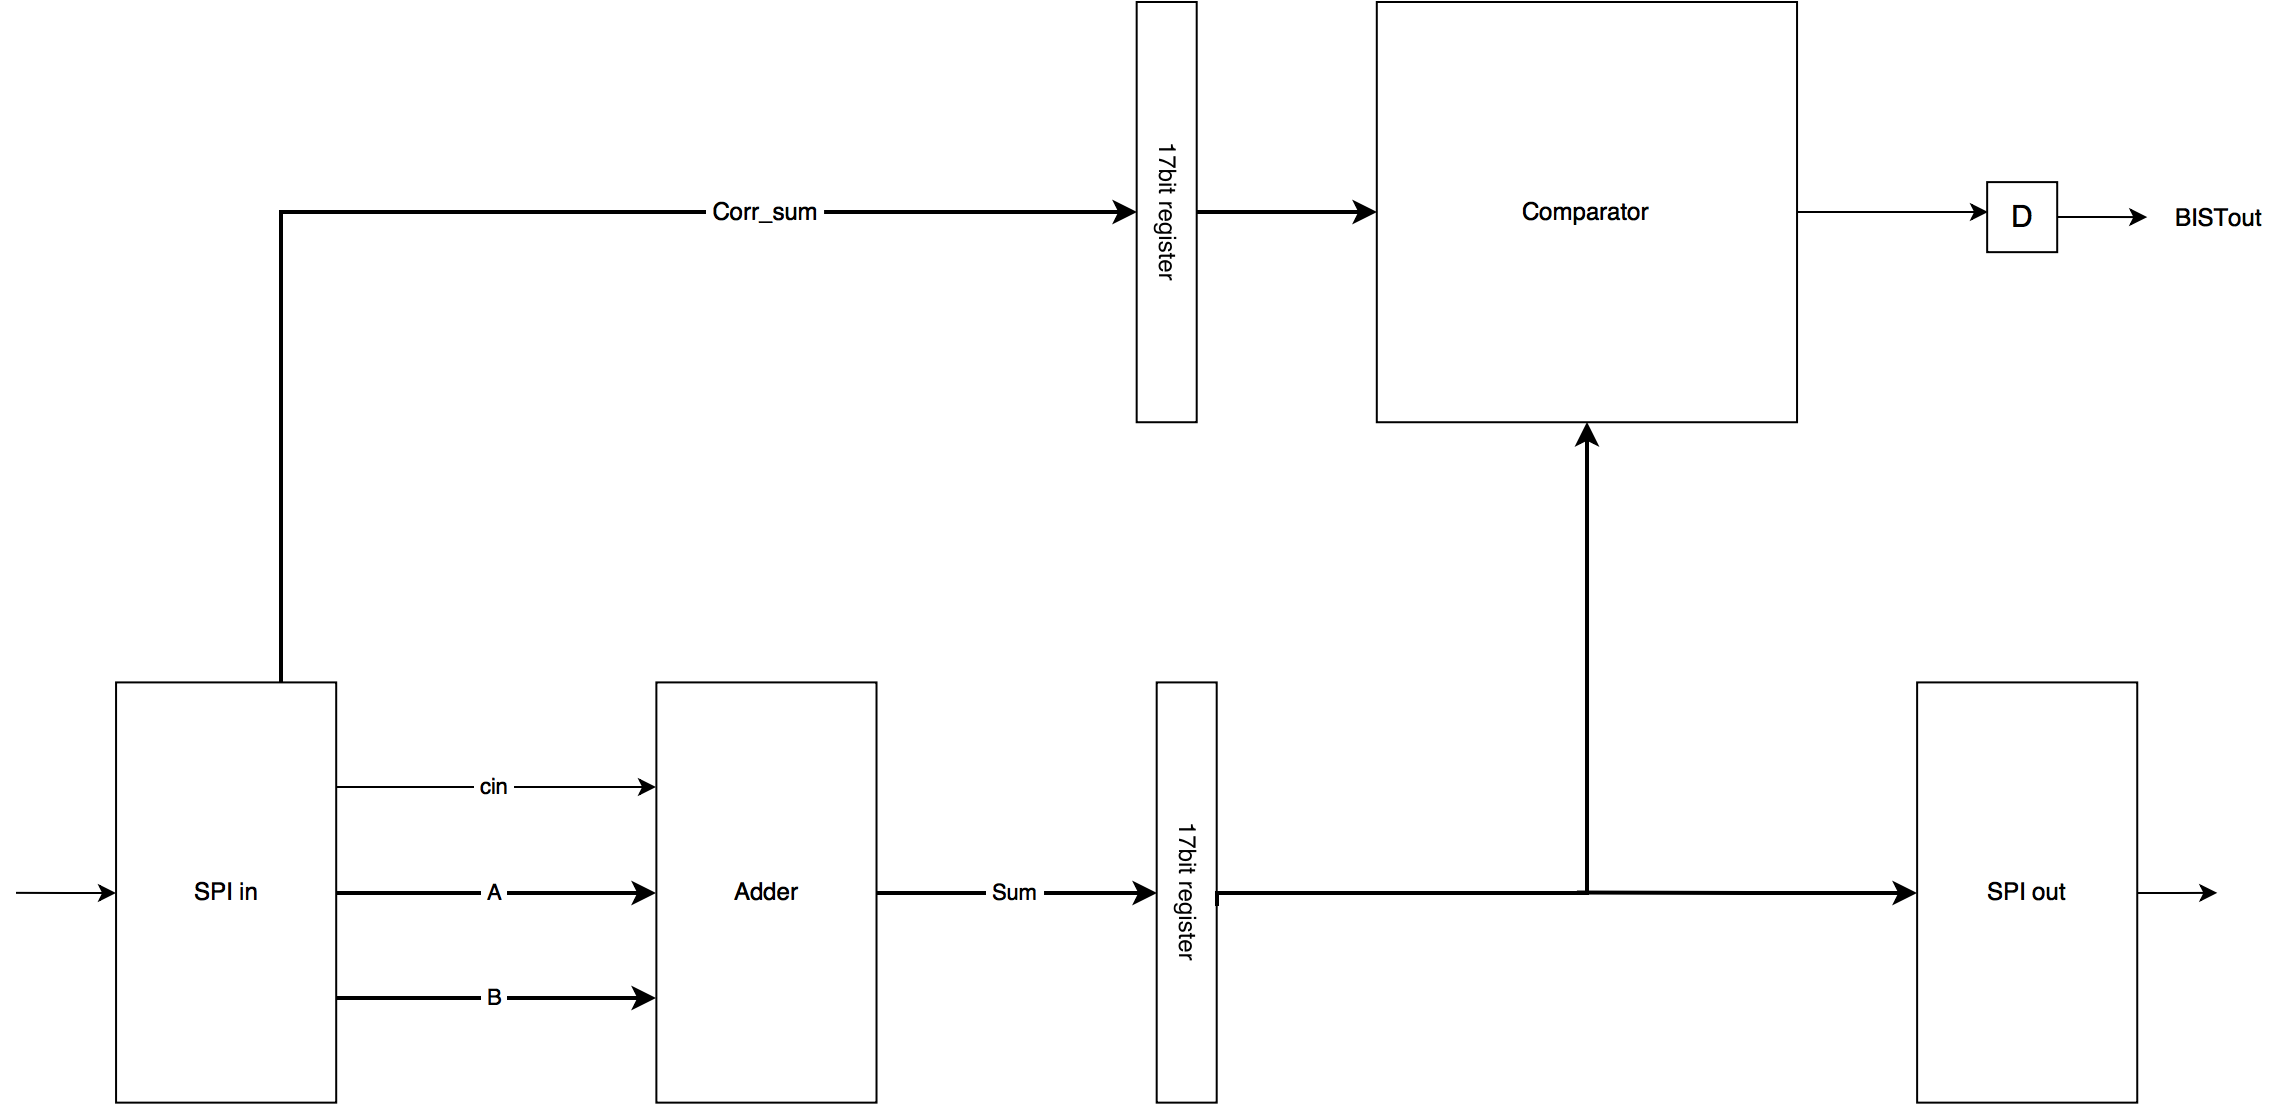
\includegraphics[scale=0.175]{../figures/top_level.png}
\caption{Block diagram of the system second iteration.}
\label{block_second}
\end{figure}

% \begin{figure}[H]
% \centering
% \captionsetup{justification=centering}
% 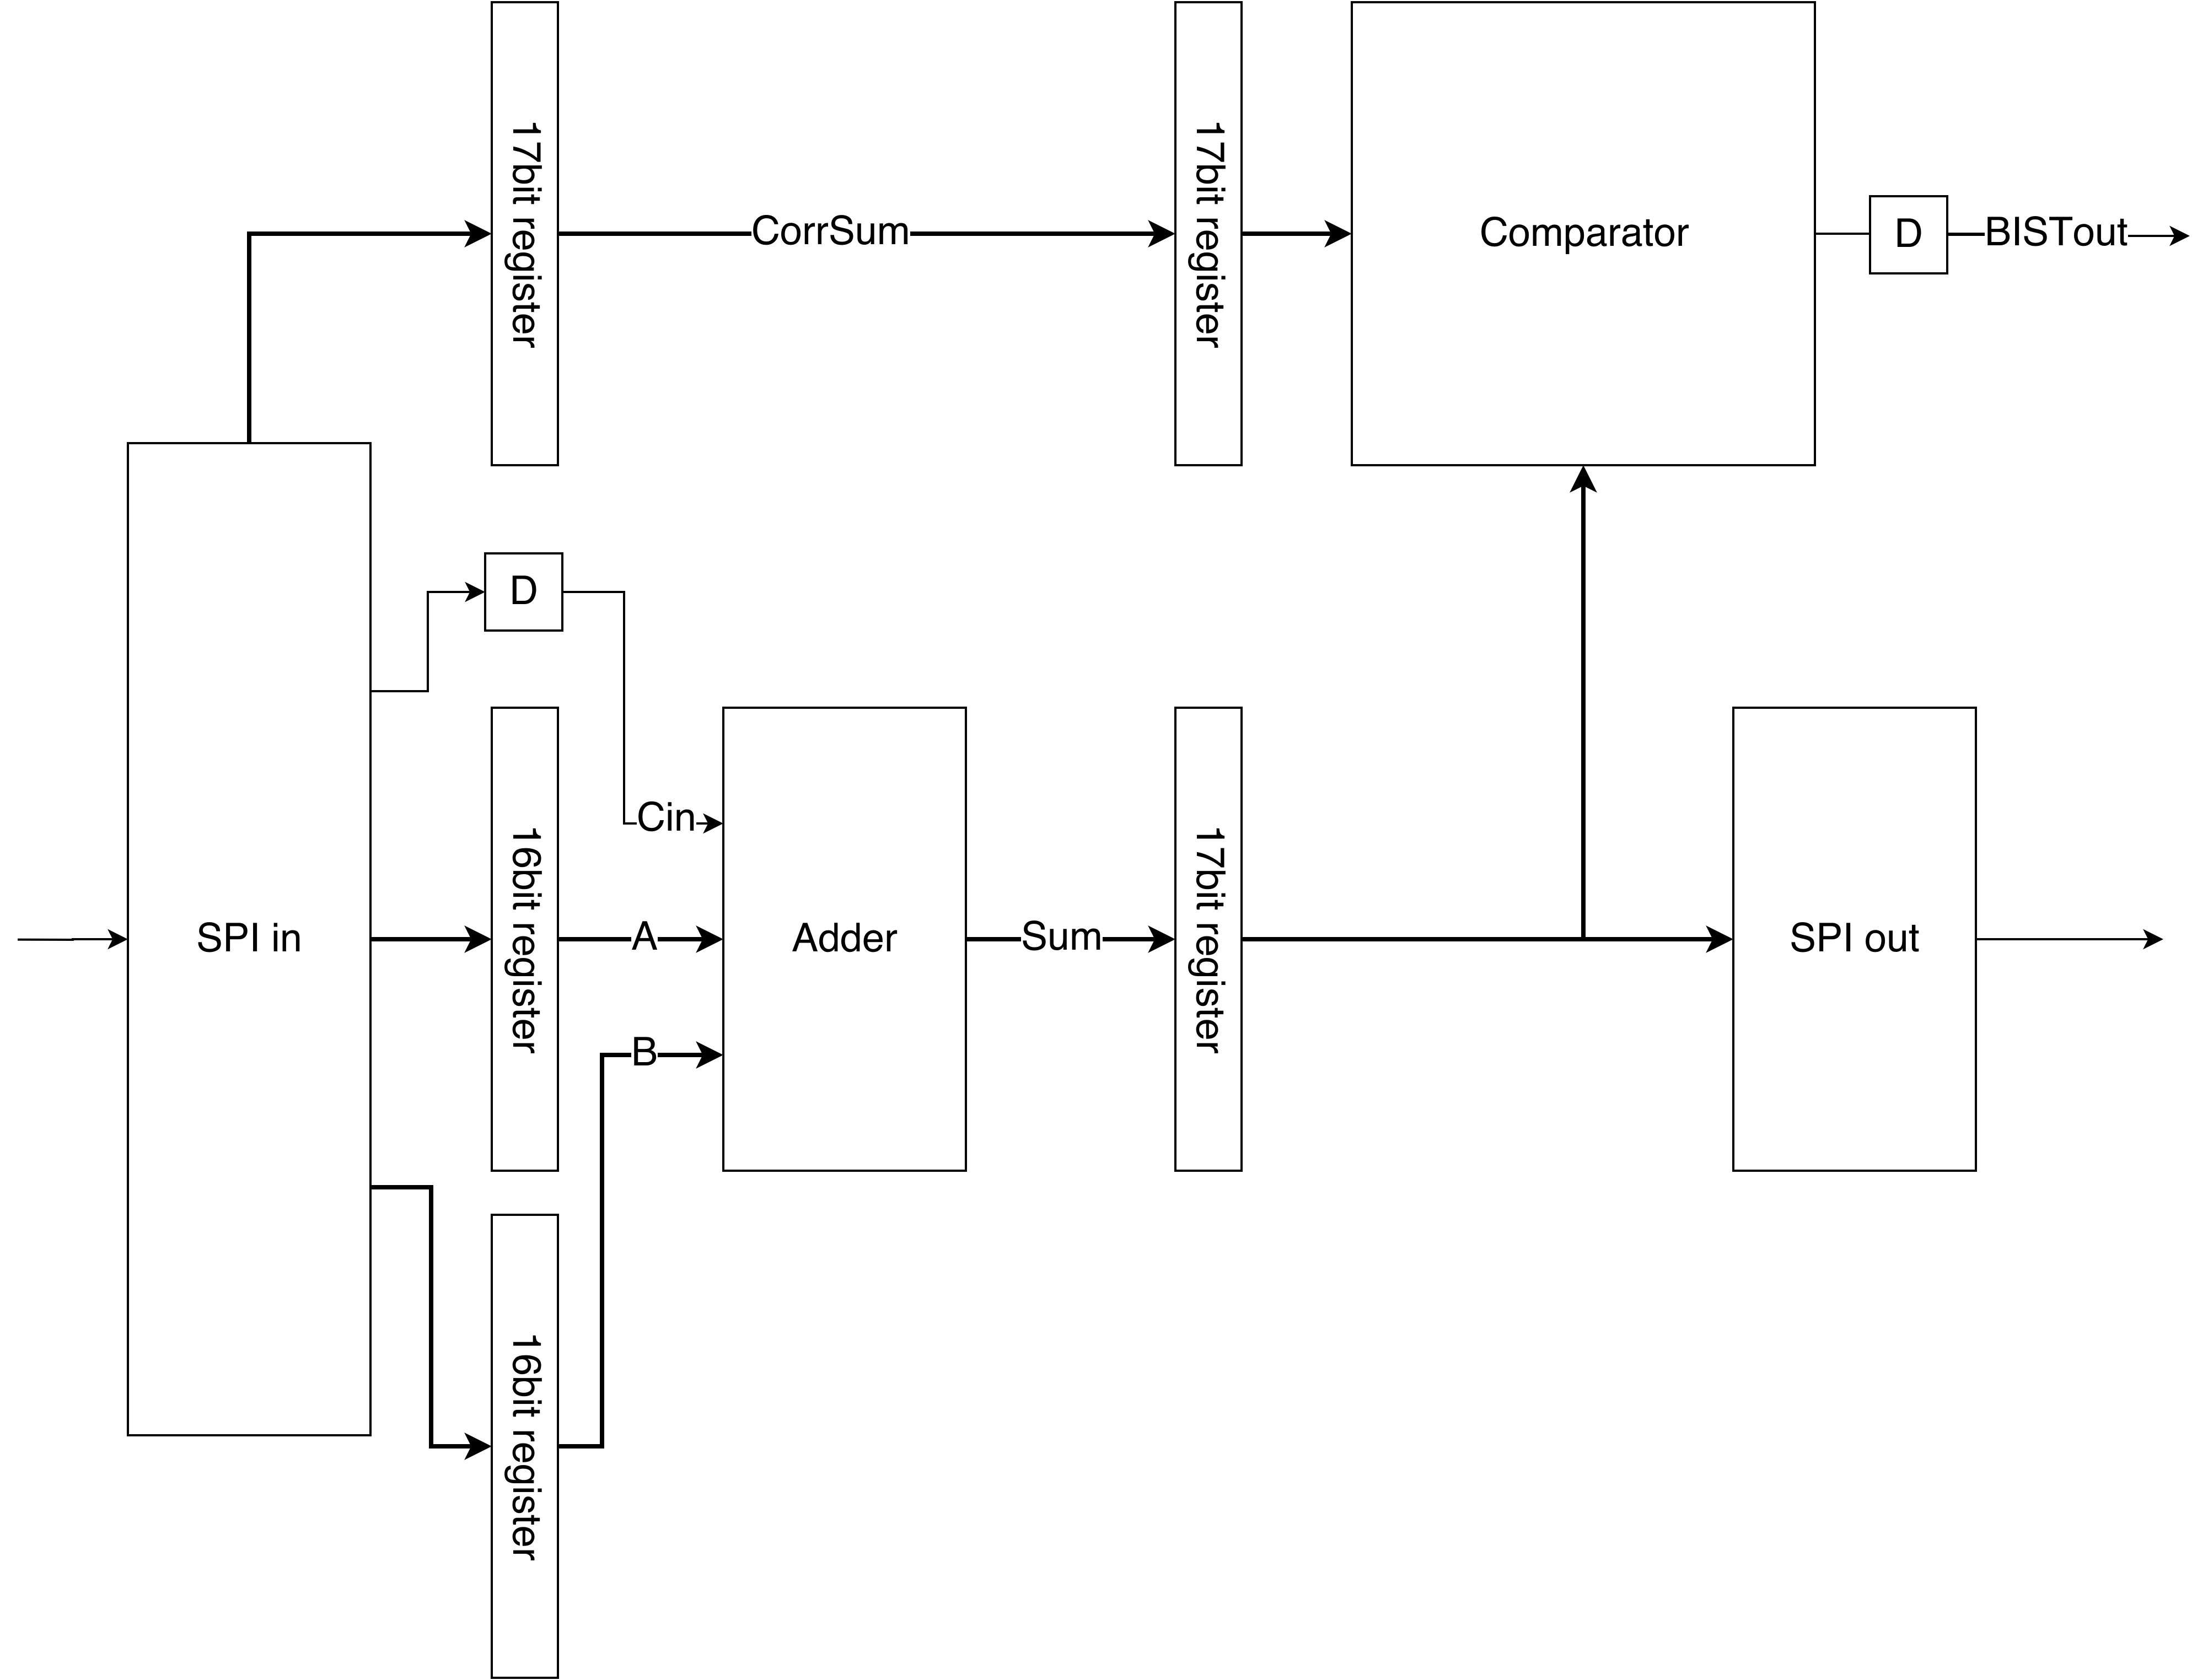
\includegraphics[scale=0.175]{../figures/top_level_final.png}
% \caption{Block diagram of the system final iteration.}
% \label{block_final}
% \end{figure}

\noindent The updated diagram contains additional registers for synchronizing the signal before and after the comparator. This was done to provide more stable signals to the comparator and to have a more easily interpreted BISTout signal. The drawback is that the BISTout signal is available two clock cycles after the addition took place which isn't very much of a problem.


\section{Simulation Results} \label{sec:simulation_results}
%This section describes the high level simulation results. As simulations with too many signals were consuming too much memory (and crashed) the group decided to only look at signals that showed if the chip worked or not.\\


%\subsection{Adder}
%In Fig. \ref{adder_sim} simulation of the propagation delay through the adder %can be seen. Due to routing problems it was shown that bit 8 of the sum were %the slowest and as can be seen, it takes approximately 2.7ns from system clock %edge until the result is ready. \\

%\subsection{SPI output}
%In Fig. \ref{spi_out_sim} the four enable signals, the spi clock and the spi enale signal from the spi output module is shown. As can be seen, the four enable signals each goes high once during the high period of the spi enable.\\
%When the spi enable signal goes low the most significant bit of the sum is available on the first falling edge of the spi clock. If you look closely, you can see that the first sum outputted are the same as the first correction sum that can be seen in table \ref{tab:test_data}. (all sums match except for the third correction sum which contains an error)\\

%\subsection{BIST}
%In Fig. \ref{bist_sim} a simulation of the BISTout signal can be seen. As mentioned earlier the correction sum contains an error which makes the BISTout signal go low for one cycle. \\
%It can also be seen that the BISTout first go high after two system clock cycles as effect from pipelining.\\

After running the simulation for different corners we retrieved the following data regarding system performance. The test data used can be seen in Tab. \ref{tab:test_data}.

\begin{table}[H]
	\caption{Corner results.}
	\centering
	\begin{tabular}{| l | c | c | c | c |}
		\hline
		Corner & Nominal & Worst speed & Worst power & Unit\\
		\hline
		Simulated temperature & $27$ & $100$ & $0$ & Celcius\\
		\hline 
		Tested frequency & $200$ & $166$ & $333$ & MHz  \\
		\hline
		Power consumption chip & $18.89$ & $16.54$ & $31.3$ & mW \\
		\hline 
		Power consumption adder & $0.93$ & $0.807$ & $1.436$ & mW \\
		\hline 
		Propagation delay sum15 & $2.209$ & $4.234$ & $1.264$ & ns \\
		\hline 
		Propagation delay cout & $2.195$ & $3.744$ & $1.332$ & ns \\
		\hline
		Possible adder frequency & $455$ & $236$ & $750$ & MHz \\
		\hline
	\end{tabular}
	\label{corner_result}
\end{table}

The propagation delay was measured between Cin and Cout and between Cin and Sum15. The possible adder frequencies in Tab. \ref{corner_result} are based on longest of these two. One thing to note is that the complete system did not function correctly during worst speed. The adder itself works fine and the correct data is outputted through SPI-out, but the built-in self test is failing.

Simulation results, for the nominal corner with a frequency of 200 MHz, of the propagation delay, the SPI-out data and of BISTout can be seen in Appendix \ref{app:simulations}.

\newpage
\section{Evaluation Plan and PAD List}
Table \ref{tab:pins} shows the pin assignments for the chip.

\begin{table}[H]
  \caption{Pin assignments}
  \centering
  \begin{tabularx}{\linewidth}{|l|l|l|X|}
    \hline
    \textbf{Name} & \textbf{Direction} & \textbf{Type} & \textbf{Description} \\ \hline
    Vdd1 & INOUT & Analog & Will provide most of the system with power and will be a steady \SI{3.3}{\volt}. \\ \hline
    Vdd2 & INOUT & Analog & Will provide the adder with power and it might vary from \SI{3.3}{\volt} downto threshold-voltage. \\ \hline
    GND &  INOUT & Analog & Ground. \\ \hline
    Clk & IN & Digital & This is the clock for the adder, some registers and control logic. Should have a frequency of at least \SI{200}{\mega\hertz} at \SI{3.3}{\volt}. Will be lower as we decrease the voltage of Vdd2. \\ \hline
    SPI\_clk & IN & Digital & This clock is used by the input and output unit and should be at least five times slower than the system clock. Should also be low if SPI\_en is inactive. \\ \hline
    SPI\_en & IN & Digital & Active low. Should go high on the first negative flank of SPI\_clk after the last value is read. \\ \hline
    SPI\_in & IN & Digital & Updates it's value as soon as SPI\_en goes low, and should have it's value ready on the first positive flank of SPI\_clk, since this is when we read the value. The value of SPI\_in should then be updated on every negative flank of SPI\_clk. \\ \hline
    SPI\_out & OUT & Digital & The data is available for read on the first falling edge of SPI\_clk after SPI\_en has gone active. \\ \hline
    BISTout & OUT & Digital & If the IN-data is correct, BISTout should be constant high after the first addition is done until the the PRBS-bit is set.  \\ \hline
    Cin & IN & Digital & Used to measure propagation delay. \\ \hline
    Cout & OUT & Analog & Used to measure propagation delay. \\ \hline
    Sum15 & OUT & Analog & Used to measure propagation delay. \\ \hline
  \end{tabularx}
  \label{tab:pins}
\end{table}


\section{Risks} \label{sec:risks}
During the transistor level design there hasn't been any considerable delays. The only thing that is an issue is that all members in the group has quite different schedules which sometimes can hinder cooperation. However the group has solved this by using good tools for project tracking (Trello) and communication (Slack). This has helped considerably with the delegation of tasks and keeping track of what needs to be done. 

During the next phase of the project, cooperation will be more important since the tasks will be harder. We will need to plan ahead and schedule occasions where we all can meet and work together.


\section{Project Evaluation} \label{sec:evaluation}
During the course of the project we gained a lot of experience related to tools, design and also cooperation. 

\subsection{Cooperation} \label{sec:eval_coop}
The group has functioned very well during the whole project except for two weeks during the beginning of the layout phase. There were some miscommunication since half of the group were on holiday the first week while the other half were on holiday during the second week of this period. This later led to some integration issues.

\subsection{Tools}
In retrospect, less time should have been spent on Verilog simulations and more time on schematic simulations. The Verilog models were very inaccurate and we had no idea what values to choose for propagation delays and rise times etc. The schematic simulations were much more accurate and at the same time quite fast. Since the simulations when doing layout were very slow, a lot of time was spent on waiting for results. Doing more design work at the schematic level would have led to more effective work and possibly a better overall design.

Another tool related issue encountered was the problem with configurations. Using configurations in Cadence seemed like a very useful feature which could help us keep a clean structure of the project by having several schematics and layouts of different verions of the same cell in one place, instead of creating several very similiar cells. It turned out however that it was very hard to maintain and the configuration editor in Cadence randomly crashed all the time when creating somewhat advanced configuations. We should have stuck to having only one schematic and one layout view in each cell, even though this led to many cells.

Quite early in the project we researched the possibility of having automatic tests of all cells in the project using a tool called Ocean. Unfortunately we could not get it to work, but it would have been very useful and could have helped us pinpoint errors with ease.

\subsection{Design}
The design work went smoothly until the integration phase. We expected some hardships during integration, but maybe not to the extent we experienced them. Things seemed to stop working for no apparent reason. Cells that worked yesterday, didn't function today and so on. Integration is hard, this is a lesson all of us will remember. 

Looking back, there are several things we could have done much better. Clock distribution, interconnects and floor planning should have been considered much earlier in the project, during the same time as when layouting the basic gates. Floor planning and interconnects could have been done much better if we would have communicated better during the early layout phase, but due to the reasons mentioned in \ref{sec:eval_coop} this didn't happen. This led to a situation were individual parts functioned well but weren't optimally adapted to eachother. For example ome components of the chip had different widths and therefore the power rails and data interconnects couldn't be aligned easily. If the floor planning had been done earlier in the layout phase, we could also have designed the basic blocks better. When we designed the basic blocks we did it almost exclusivly using metal 1 and 2 layers, in order to leave room for power supply and clock signals on metal 3 and 4 layers. If we would have considered the power supply and clock signals at the same time as when we designed the basic blocks, we could probably have ended up with a tighter design.

Late in the project we discovered some timing issues probably related to the SPI control logic, but we didn't have time to make a new easier and faster control logic design since the layout was already done and the simulations took considerable time. If we had done more testing in the schematic stage, with more realistic loads and possible doing worst case corner testing in schematic simulations, this problem would have been discovered earlier and the control logic could have been redesigned. The problem was eventually solved without a new design but not in an optimal way.


\newpage

\begin{appendix}

\section{Simulation results}
\label{app:simulations}
% \subsection{SPI In}
% \begin{figure}[H]
%   \centering
%   \captionsetup{justification=centering}
%   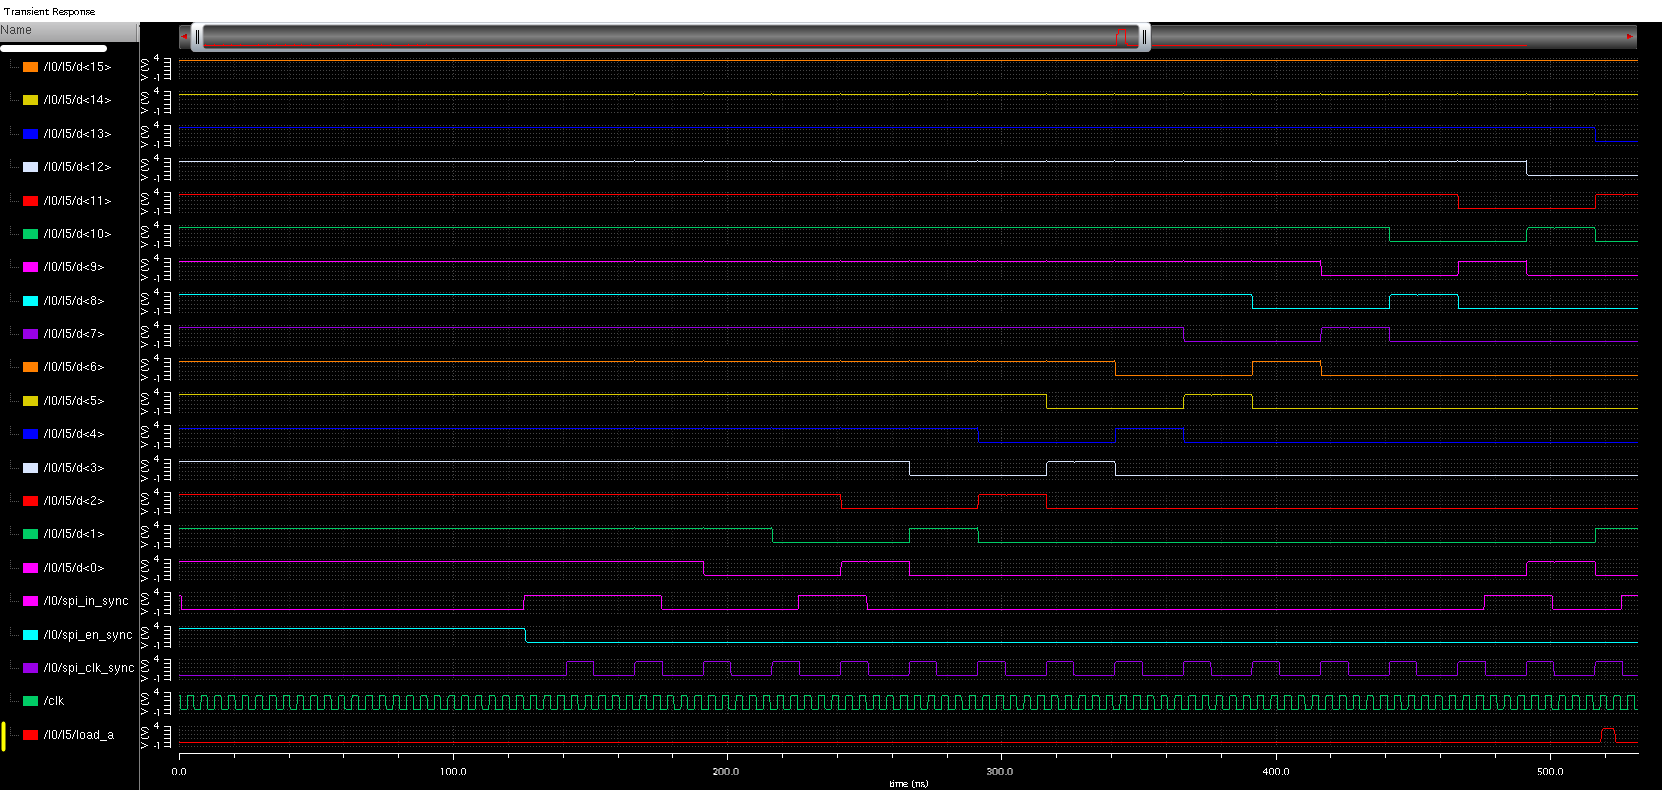
\includegraphics[angle=90, scale=0.44]{../figures/test2_spi_in}
%   \caption{SPI receiver} 
% \end{figure}

% \begin{figure}[H]
%   \centering
%   \captionsetup{justification=centering}
%   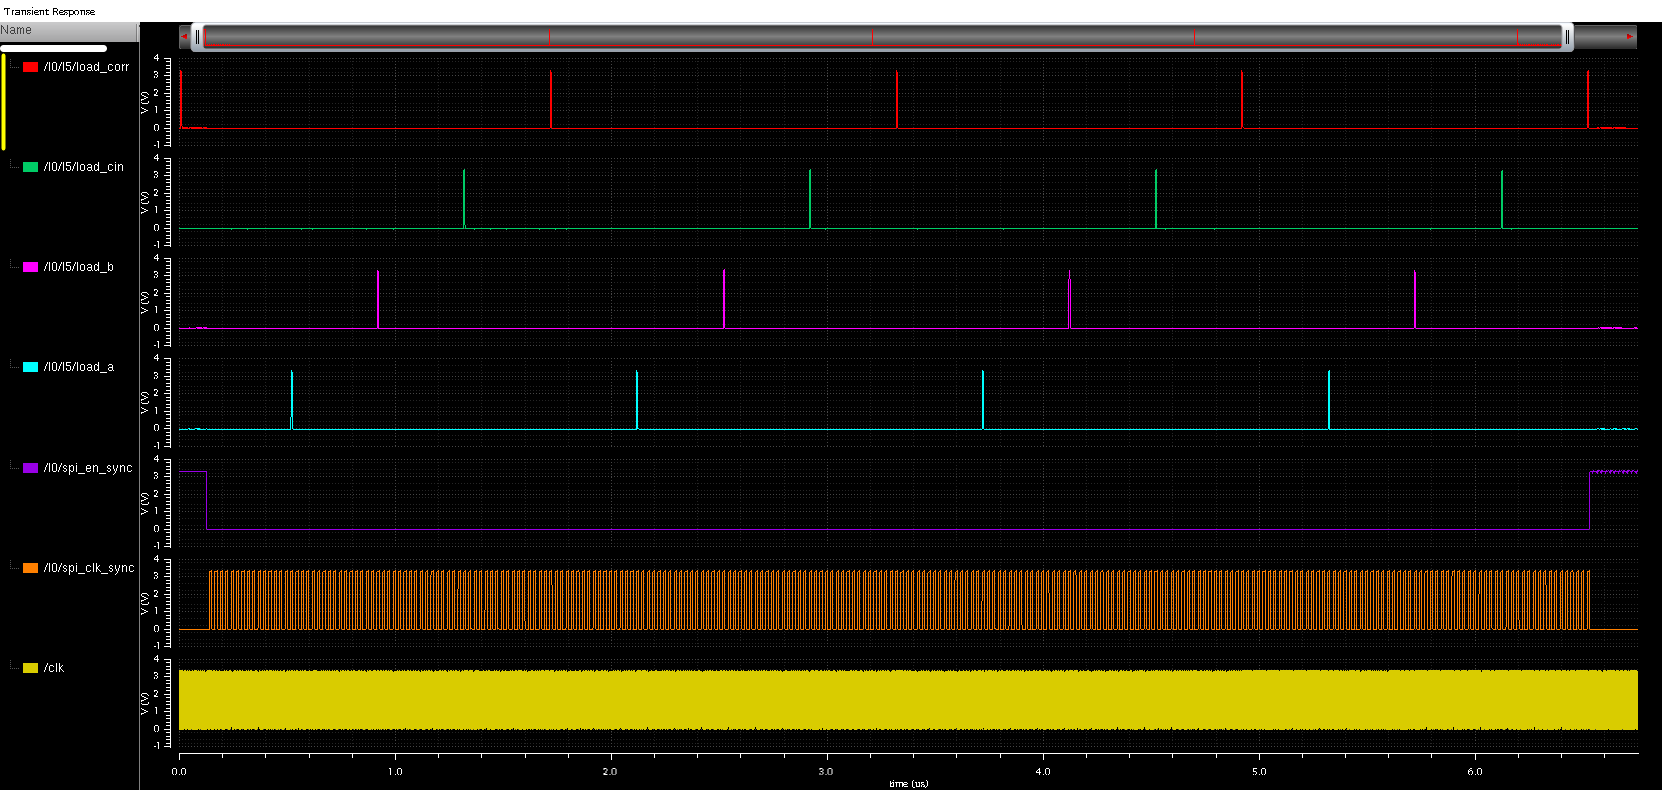
\includegraphics[angle=90, scale=0.46]{../figures/test2_spi_load}
%   \caption{Load signals}
% \end{figure}

% \begin{figure}[H]
%   \centering
%   \captionsetup{justification=centering}
%   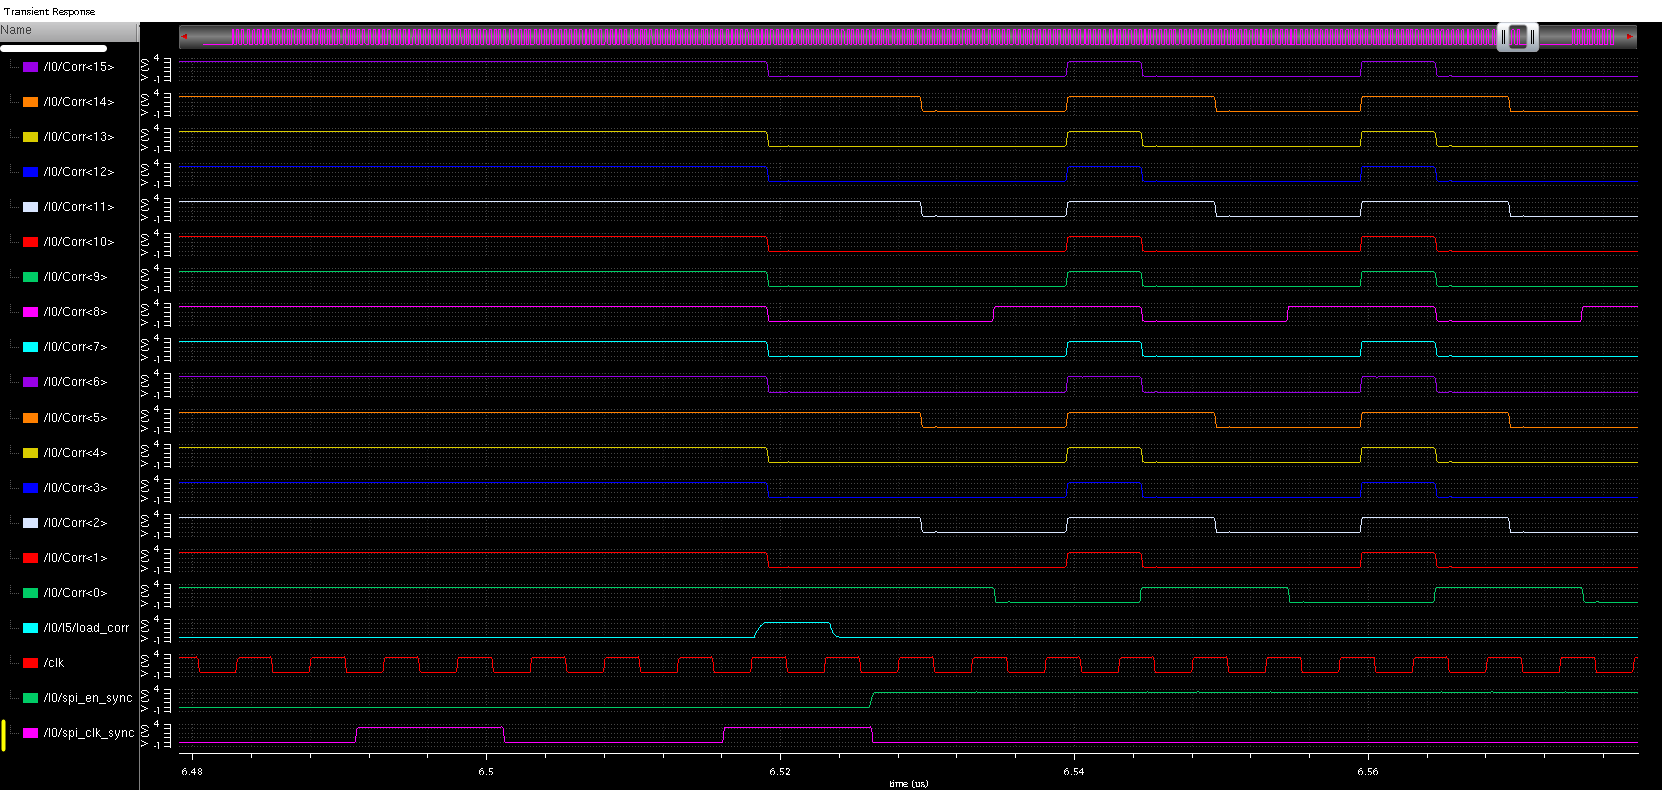
\includegraphics[angle=90, scale=0.46]{../figures/test2_spi_abc}
%   \caption{PRBS registers}
% \end{figure}

% \subsection{SPI Out}

% \begin{figure}[H]
%   \centering
%   \captionsetup{justification=centering}
%   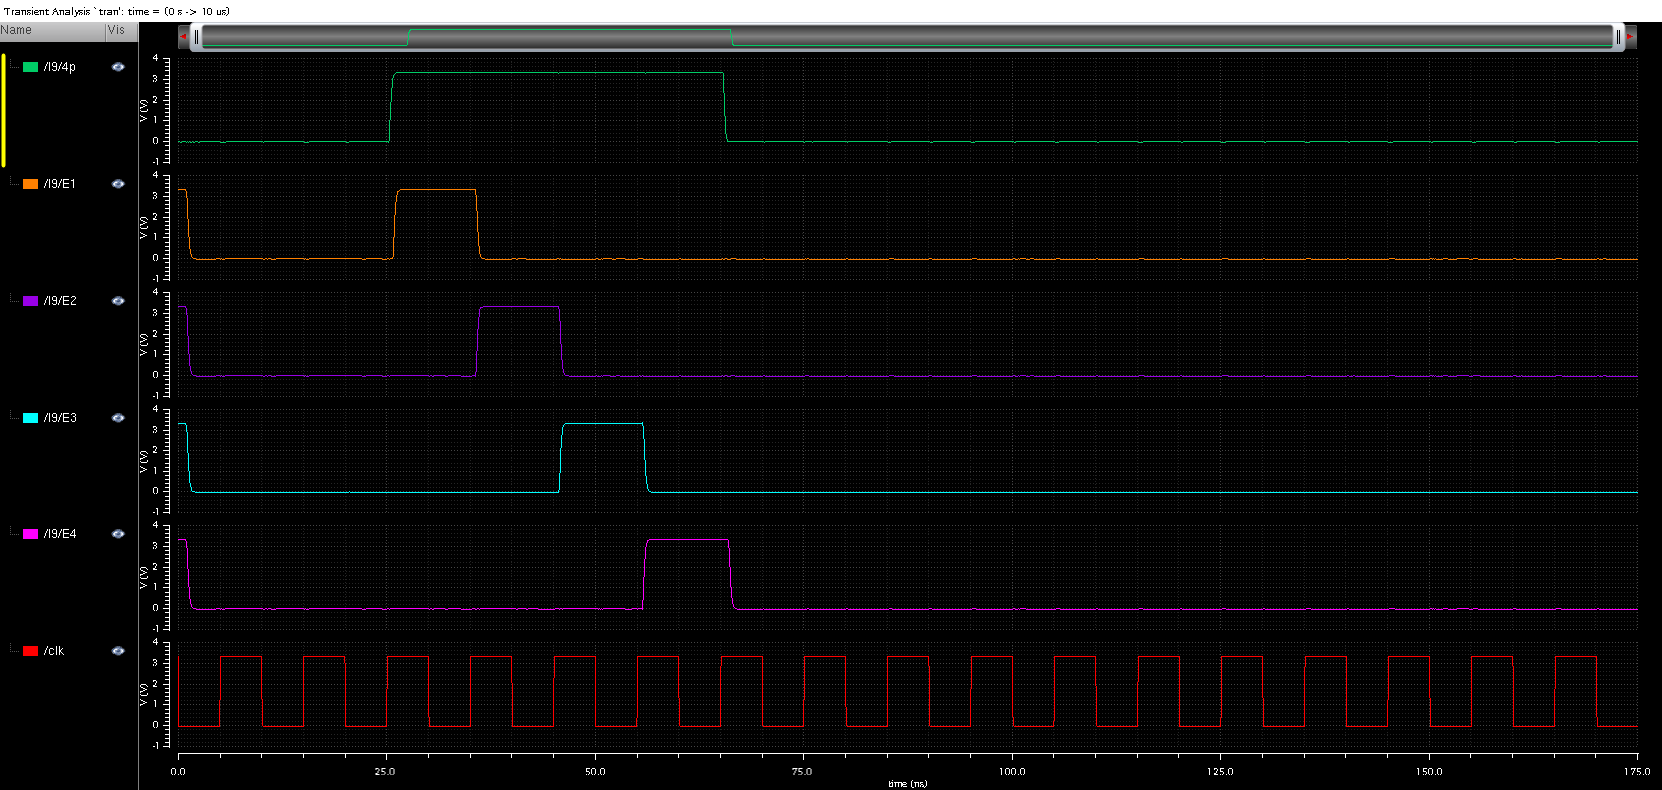
\includegraphics[angle=0, scale=0.55]{../figures/spi_out_control}
%   \caption{Enable high} \label{fig:spi_out1}
% \end{figure}

% \begin{figure}[H]
%   \centering
%   \captionsetup{justification=centering}
%   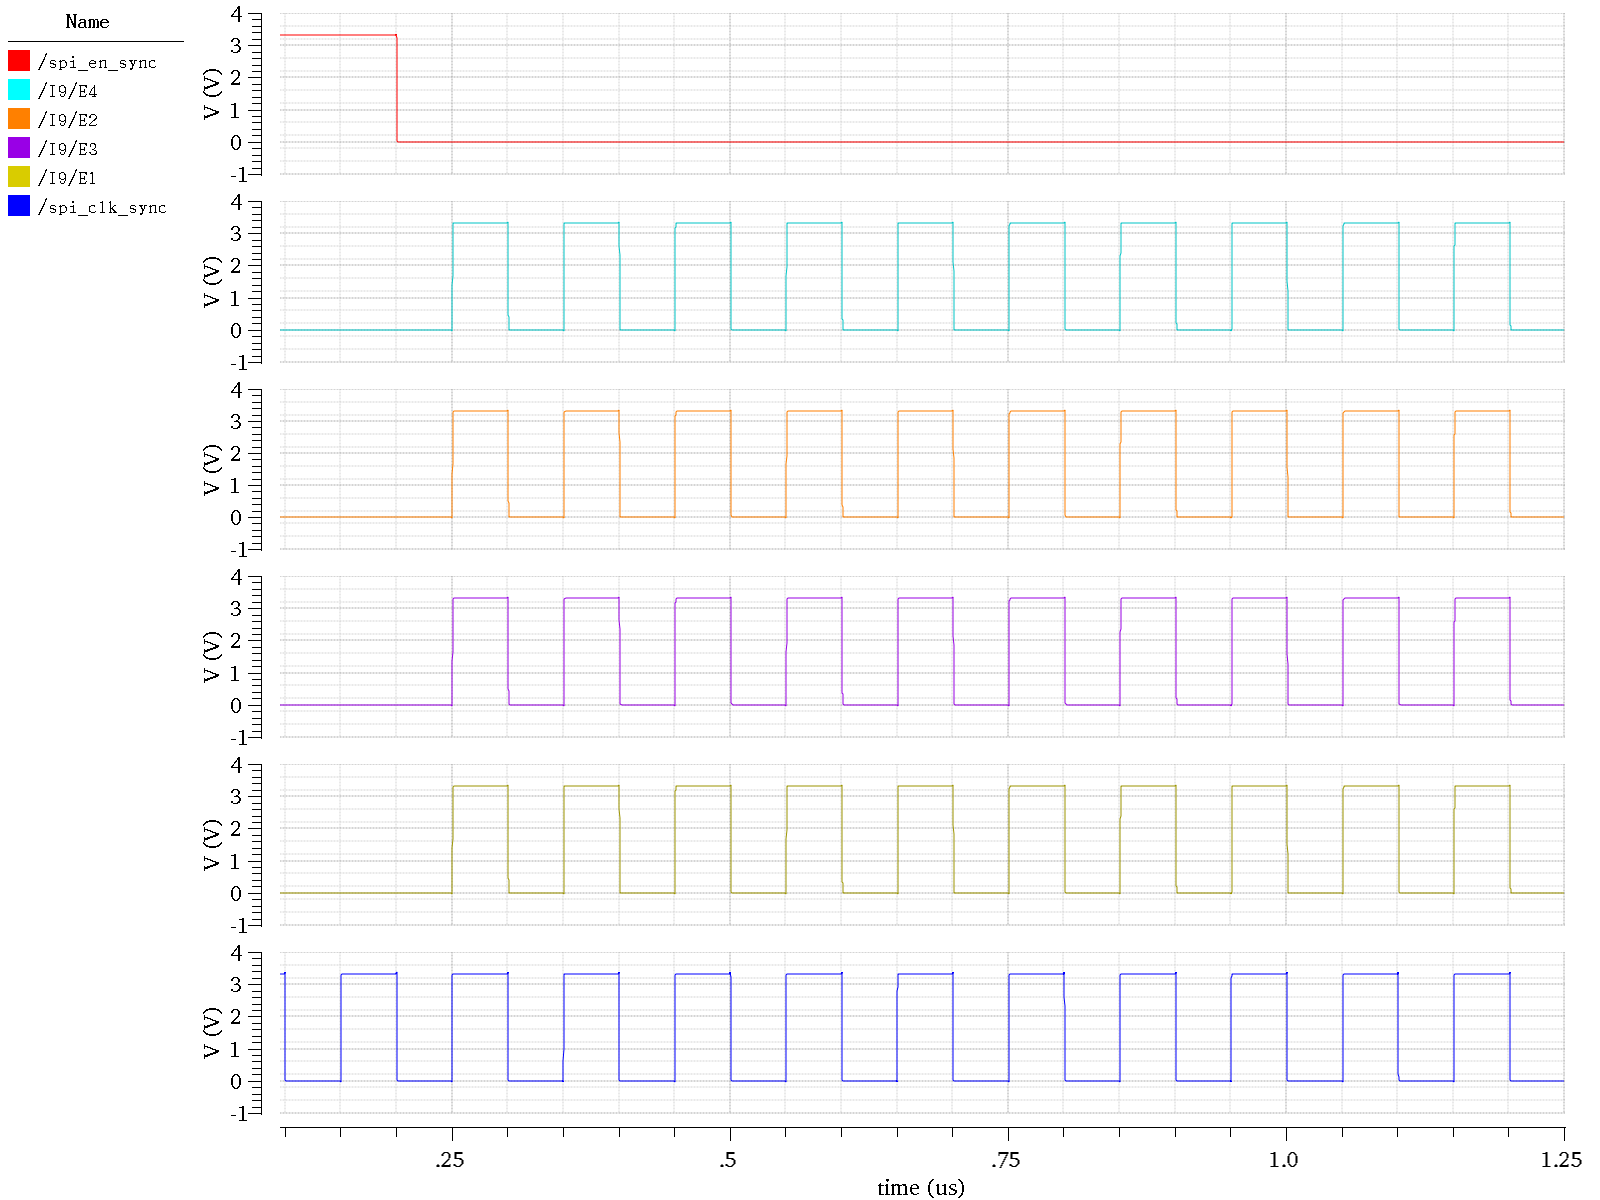
\includegraphics[angle=0, scale=0.55]{../figures/spi_out_control2}
%   \caption{Enable low} \label{fig:spi_out2}
% \end{figure}

% \subsection{Adder}

% \begin{figure}[H]
%   \centering
%   \captionsetup{justification=centering}
%   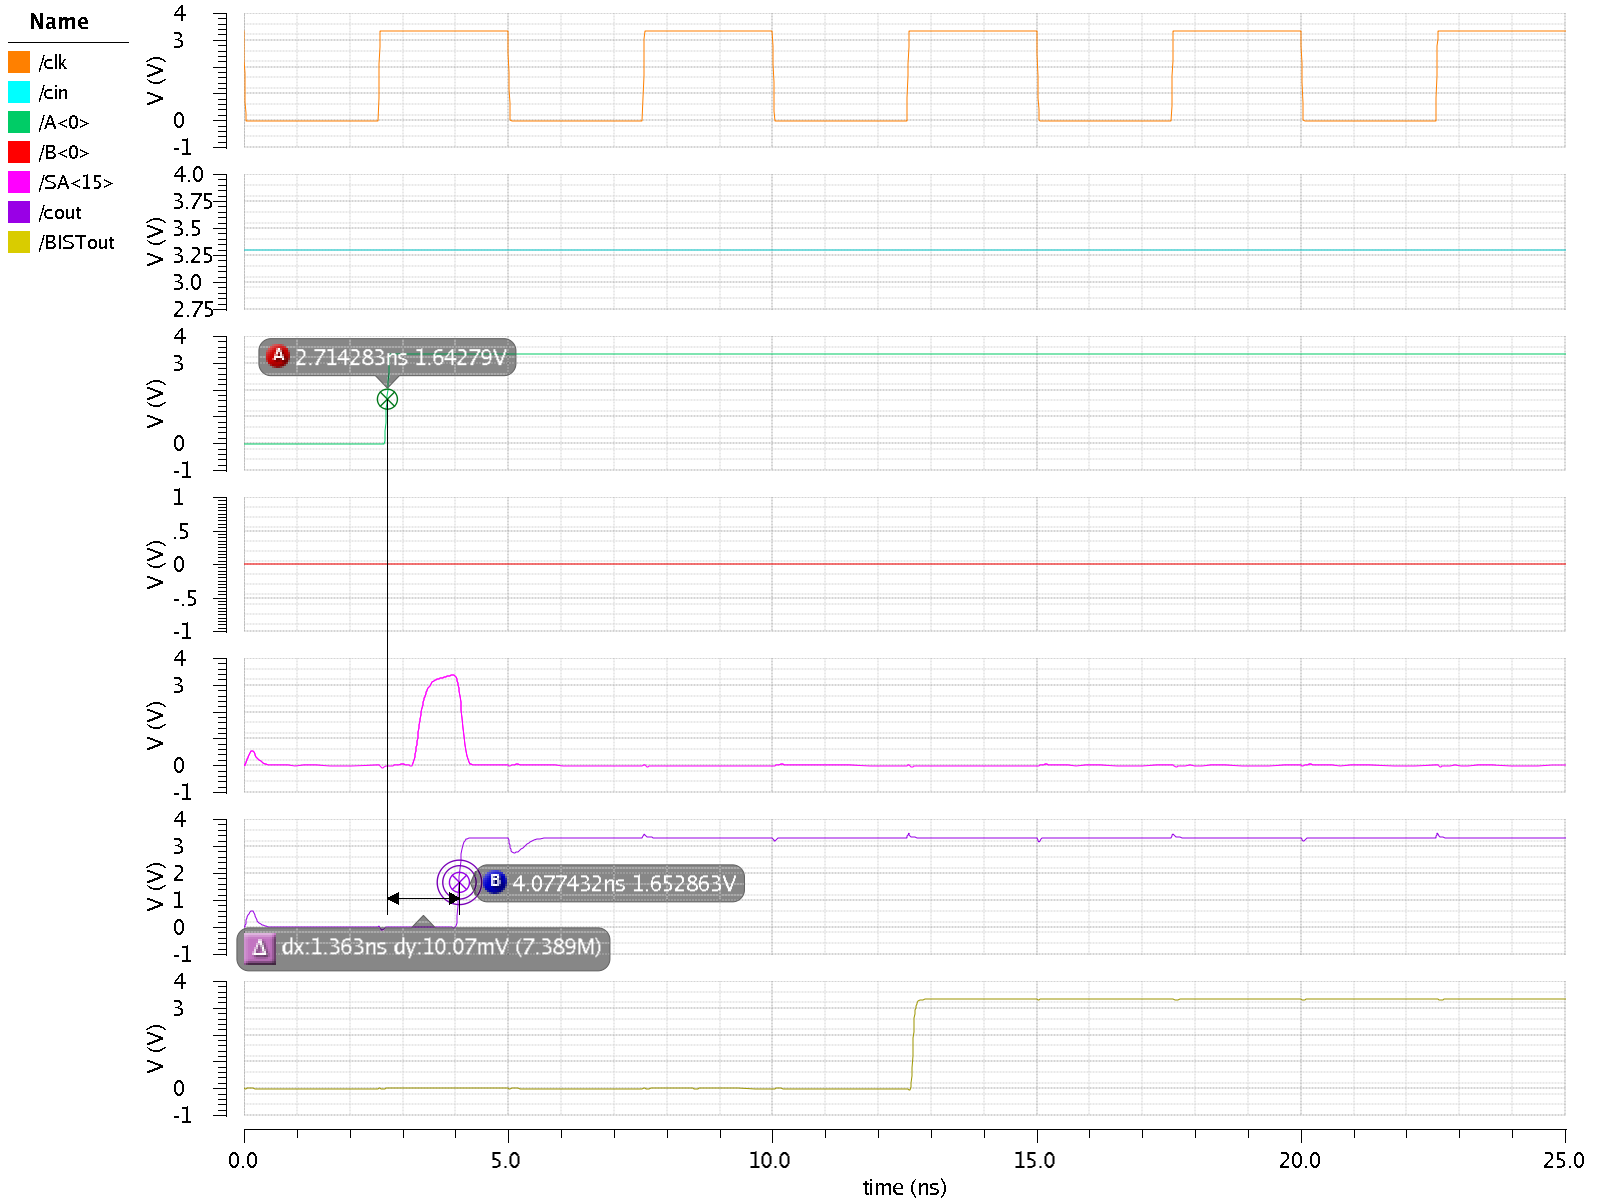
\includegraphics[angle=90, scale=1]{../figures/kogge_delay}
%   \caption{Worst case propagation delay Kogge-Stone Adder} \label{fig:kogge_delay}
% \end{figure}



\end{appendix}
\end{document}
